% Machine translated from the Danish original, ../danish/ad-problems-march-2025.tex
\noindent\emph{This problem set has been machine translated from the Danish original.}
\medskip

\section*{Multiple-choice}\label{sec:mc}

\placeholder{Where to enter the multiple-choice answers, e.g.\ the multiple-choice module of the exam system.}

\multiplechoicestart

\question{Recurrences}
Which of the following recurrences, assuming $T(n)=1$ for $n\leq 1$, have the solution $T(n)=\Theta(n \log n)$? \multipleanswers
\optionsstart
\answer $T_1(n) = 3\cdot T_1(n/3) + \Theta(n)$ \correct
\answer $T_2(n) = T_2(n/2) + \Theta(n \log n)$ \correct
\answer $T_3(n) = 3\cdot T_3(n/4) + \Theta(n)$
\answer $T_4(n) = 2\cdot T_4(n/2) + \Theta(1)$
\answer $T_5(n) = 4\cdot T_5(n/2) + \Theta(n)$
\answer $T_6(n) = T_6(n-1) + \Theta(\log n)$ \correct
\optionsend
\explanation{The recurrence $T_1$ is solved by the master theorem to give $\Theta(n \log n)$, and for $T_2$, with $a=1$, $b=2$ and $f(n)=\Theta(n \log n)$, the same growth rate is obtained. The other recurrences have different solutions, which can be found using the master theorem.}

\question{Recursive algorithms}
A recursive algorithm \(A\) works as follows on an input \(x\) of size \(n\):
\begin{itemize}
  \item If \(n=1\), an answer is returned in time \(\Theta(1)\).
  \item Otherwise:
  \begin{itemize}
    \item Time \(\Theta(n)\) is spent computing two partial results \(x_1\) and \(x_2\), each of size \(n-1\).
    \item The algorithm is called recursively on \(x_1\) and \(x_2\), after which the answers \(y_1\) and \(y_2\) are received.
    \item The answers \(y_1\) and \(y_2\) are combined into an answer in time \(\Theta(1)\).
  \end{itemize}
\end{itemize}
Which recurrence best describes the running time \(T(n)\) of the algorithm \(A\), with base case \(T(1)=1\)?
\oneanswer
\optionsstart
\answer \(T(n)=2\,T(n/2)+\Theta(1)\)
\answer \(T(n)=2\,T(n/2)+\Theta(n)\)
\answer \(T(n)=2\,T(n/2)+\Theta(2^n)\)
\answer \(T(n)=2\,T(n-1)+\Theta(1)\)
\answer \(T(n)=2\,T(n-1)+\Theta(n)\) \correct
\answer \(T(n)=2\,T(n-1)+\Theta(2^n)\)
\optionsend
\explanation{Two recursive calls are made on inputs of size \(n-1\), and in addition $\Theta(n)$ time is spent computing the two partial results and $\Theta(1)$ time combining them, which in total gives $\Theta(n)$. Hence we get the recurrence \(T(n)=2T(n-1)+\Theta(n)\).}

\question{Invariants}
Consider this algorithm, which takes as input an array $A[1:n]$ of integers and an integer $k$.
\begin{codebox}
\Procname{$\proc{Two-Sum-BruteForce}(A, n, k)$}
\li \For $i \gets 1$ \To $n-1$
\li \Do
        \For $j \gets i+1$ \To $n$
\li     \Do
            \If $A[i] + A[j] = k$
\li         \Then \Return \const{True}
         \End
        \End
    \End
\li \Return \const{False}
\end{codebox}
Which of the following invariants hold (for every input) at the \emph{beginning} of each iteration of the outer loop?
In the successive iterations the variable $i$ takes the values $1, 2, \dots$, and the invariant is evaluated with respect to the current value of $i$ during the given iteration.
The invariant need not hold if line 4 is executed and the iteration is therefore interrupted.
\multipleanswers
\optionsstart
\answer For all $i',j'$ with $1\leq i' < i$ and $1\leq j'<i$ we have $A[i']+A[j'] = k$
\answer For all $i',j'$ with $1\leq i' < i$ and $1\leq j'<i$ we have $A[i']+A[j'] \ne k$
\answer For all $i',j'$ with $1\leq i' < i$ and $j'\in\{1,\dots,n\}\backslash\{i'\}$ we have $A[i']+A[j'] = k$
\answer For all $i',j'$ with $1\leq i' < i$ and $j'\in\{1,\dots,n\}\backslash\{i'\}$ we have $A[i']+A[j'] \ne k$ \correct
\optionsend
\explanation{In iteration $i$ the algorithm checks whether there is some $j$ such that $A[i]+A[j]=k$. Pairs of indices that have already been checked are skipped by starting the inner loop at $j=i+1$. Therefore invariant 4 is true. Invariants 1 and 3 fail after at most two iterations if, e.g., $A = \langle 0, 0, 0\rangle$ and $k=1$. Invariant 2 fails if there exists $j'$ with $A[j'] = k/2$, since in the case $i'=j'$ we then have $A[i']+A[j'] = k$.}

\question{Enigma}
Consider this algorithm, which takes as input an array $A[1:n]$ and two indices $i,j$ with $i\leq j$, and which modifies the array $A$.
\begin{codebox}
  \Procname{$\proc{Enigma}(A, i, j)$}
  \li \If $j\leq i+1$ \textbf{ and } $A[j]<A[i]$ \Do
  \li swap $A[i]$ with $A[j]$  \li \ElseIf $j>i+1$ \Do
  \li $\proc{Enigma}(A,i,j-1)$
  \li $\proc{Enigma}(A,i+1,j)$
  \li $\proc{Enigma}(A,i,j-1)$
  \End
\end{codebox}
Which of the following statements hold when we call $\proc{Enigma}(A, 1, n)$?
%, where $A$ is an array of length~$n$?
\multipleanswers
\optionsstart
\answer The algorithm generates all permutations of the numbers in $A$ before it terminates.
\answer The algorithm sorts $A$ in nondecreasing order.\correct
\answer The algorithm sorts $A$ in nonincreasing order.
\answer The running time is $\Theta(n \log n)$.
\answer The running time is $\Theta(n^3)$.
\answer The running time is $\Theta(3^n)$.\correct
\answer The running time is $\Theta(n!)$.
\optionsend
\explanation{The algorithm sorts $A$ in nondecreasing order, which can be seen by a proof by induction. After the first two recursive calls, the maximum element is in the last position. Therefore the last recursive call suffices to complete the sorting. The running time satisfies the recurrence $T(n) = 3 T(n-1) + O(1)$, which can be solved by the substitution method to give $\Theta(3^n)$ time.}

\question{Work and span}
Consider this parallel algorithm, which counts the number of nodes in a binary tree, given by its root node $T$.
A node $T$ has children $T.left$ and $T.right$, where the value $\proc{nil}$ is used to indicate the empty tree.

\begin{codebox}
\Procname{$\proc{Parallel-InOrder-Count}(T)$}
\li \If $T = \proc{nil}$
\li \Then \Return $0$
\li \Else
%\li     $leftCount \gets 0$
%\li     $rightCount \gets 0$
\li     \Spawn $leftCount \gets \proc{Parallel-InOrder-Count}(T.\id{left})$
\li     $rightCount \gets \proc{Parallel-InOrder-Count}(T.\id{right})$
\li     \Sync
\li     \Return $leftCount + rightCount + 1$
\end{codebox}
If the tree with root node $T$ has $n$ nodes and height $h$, what are the work and span of the algorithm?
\oneanswer
\optionsstart
\answer Work $T_1=\Theta(n)$, span $T_\infty=\Theta(\log h)$
\answer Work $T_1=\Theta(n)$, span $T_\infty=\Theta(\log n)$
\answer Work $T_1=\Theta(n)$, span $T_\infty=\Theta(h)$ \correct
\answer Work $T_1=\Theta(h)$, span $T_\infty=\Theta(\log h)$
\answer Work $T_1=\Theta(h)$, span $T_\infty=\Theta(\log n)$
\answer Work $T_1=\Theta(h)$, span $T_\infty=\Theta(h)$
\optionsend
\explanation{The recursive calls are executed in parallel, and everything else takes constant time. Therefore the span of the algorithm is proportional to the recursion depth $h$. The work is proportional to the number of nodes, since the algorithm spends constant time on each node.}

\question{Parallel algorithms}
Suppose that a parallel algorithm on inputs of size $n$ has work $T_1=\Theta(n \log n)$ and span $T_\infty=\Theta(n)$.
We are interested in the time $T_P$ used to run the algorithm on $P$ processors with greedy scheduling.
Which of the statements below are correct?
\multipleanswers
\optionsstart
\answer If $P = \Theta(1)$ then $T_P = O(n^2)$ \correct
\answer If $P = \Theta(\log{n})$ then $T_P = O(n)$ \correct
\answer If $P = \Theta(\sqrt{n})$ then $T_P = O(\sqrt{n})$
\answer If $P = \Theta(n)$ then $T_P = O(\log n)$
\answer If $P = \Theta(n \log n)$ then $T_P = O(1)$
\optionsend
\explanation{By CLRS Theorem 26.1, $T_P \leq T_1 / P + T_\infty$, and by Theorem 26.2 this bound is within a factor of 2 of the true running time. Substituting the values of $P$ we get the following bounds: 1. $T_P = \Theta(n \log n + n) = \Theta(n \log n)$, 2. $T_P = \Theta(n \log(n)/\log n + n) = \Theta(n)$, 3. $T_P = \Theta(n \log(n)/\sqrt{n} + n) = \Theta(n)$, 4. $T_P = \Theta(n \log(n) / n + n) = \Theta(n)$, 5. $T_P = \Theta(n \log(n) / (n \log n) + n) = \Theta(n)$. This implies bound 1.\ and matches bound 2., but is worse than the bounds in 3., 4.\ and 5.
}

\pageshift

\question{Invariants for dynamic tables}
Consider dynamic tables as described in CLRS Section 16.4.2, i.e., the version with a {\sc Table-Delete} operation.
Which of the following statements are valid invariants that hold after every {\sc Table-Insert} and {\sc Table-Delete} operation?
Note that the possible invariants are not independent: we have $1 \Rightarrow 2 \Rightarrow 3$ and $4 \Rightarrow 5 \Rightarrow 6$.
\multipleanswers
\optionsstart
\answer $T.size \leq T.num$
\answer $T.size \leq 2\cdot T.num$
\answer $T.size \leq 4\cdot T.num$ \correct
\answer $T.num \leq T.size$ \correct
\answer $T.num \leq 2\cdot T.size$ \correct
\answer $T.num \leq 4\cdot T.size$ \correct
\optionsend
\explanation{The operations are implemented such that the number of elements $T.num$ can vary between 25\% and 100\% of the table's capacity, $T.size$.
Options 5 and 6 give loose upper bounds but are nevertheless valid invariants.}

\question{Time complexity of Fibonacci heaps}
Suppose that a {\sc Fib-Heap-Decrease-Key} operation is performed on a Fibonacci heap $H$ with $n$ keys, as described in CLRS online Chapter 19.
The actual time used by the operation is not necessarily the same as the amortized time.
Let the potential function have the value $\Phi(H)$ before the operation and $\Phi(H')$ after the operation.
What can we say with certainty about the actual time used by this single {\sc Fib-Heap-Decrease-Key} operation?
\multipleanswers
\optionsstart
\answer The time is $O(1)$
\answer The time is $O(\log n)$
\answer The time is $O(n)$ \correct
\answer The time is $O(1 + \Phi(H') - \Phi(H))$
\answer The time is $O(1 + \Phi(H) - \Phi(H'))$ \correct
\optionsend
\explanation{The amortized analysis of {\sc Fib-Heap-Decrease-Key} shows that the operation runs in $O(1)$ amortized time, where the precise time used can be expressed as $O(1 + \Phi(H) - \Phi(H'))$.
The running time is bounded by the number of ``cascading cuts'', which is $O(n)$ but not necessarily $O(1)$ or $O(\log n)$.
The value $\Phi(H') - \Phi(H)$ can be a negative number of magnitude $\Omega(n)$, so option 4 is not correct.
}

\question{Rod cutting}
Consider the algorithm \textsc{Extended-Bottom-Up-Cut-Rod} as described in CLRS Section 14.1.
On an unknown input, the algorithm returns a vector $r$ of values and a vector $s$ of rod lengths:
\[
r=\langle 0, 3, 6, 10, 13, 16, 20, 23, 26\rangle
\]
\[
s=\langle 1, 1, 3, 1, 1, 3, 1, 1 \rangle
\]
How many rods are there in the optimal solution that can be computed from $r$ and $s$?
\oneanswer
\optionsstart
\answer 2 rods
\answer 3 rods
\answer 4 rods \correct
\answer 10 rods
\answer 16 rods
\answer 26 rods
\optionsend
\explanation{The lengths can be read off from $s$. $s[8]$ says that we should start with a rod of length 1, entry $s[7]$ says that the next rod also has length 1, entry $s[6]$ says that the next rod has length 3, and entry $s[3]$ says that the last rod has length 3. That is,~four rods in total.}

\question{Longest common subsequence}
We consider the longest common subsequence algorithm in CLRS Section 14.4, run on the strings SMOOTH and MOTOR.
What should the contents of the two cells marked {\bf X} and {\bf Y} be?

\begin{center}
\begin{tabular}{c|c|c|c|c|c|c|c||}
    &   & S & M & O & O & T & H\\
    \hline
     & 0 & 0 & 0 & 0 & 0 & 0 & 0\\
     \hline
    M & 0 & $\uparrow0$ & $\nwarrow1$ & $\leftarrow1$ & $\leftarrow1$ & $\leftarrow1$ & $\leftarrow1$ \\
    O & 0 & $\uparrow0$ & $\uparrow1$ & $\nwarrow2$ & $\nwarrow2$ & $\leftarrow2$ & $\leftarrow2$ \\
    T & 0 & $\uparrow0$ & $\uparrow1$ & $\uparrow2$ & $\uparrow2$ & $\nwarrow3$ & $\leftarrow3$ \\
    O & 0 & $\uparrow0$ & $\uparrow1$ & {\bf X} & $\nwarrow3$ & $\uparrow3$ & $\uparrow3$ \\
    R & 0 & $\uparrow0$ & $\uparrow1$ & $\uparrow2$ & $\uparrow3$ & $\uparrow3$ & {\bf Y} \\
    \hline
\end{tabular}
\end{center}

\oneanswer
\optionsstart
\answer $X = \leftarrow2$, $Y = \uparrow3$
\answer $X = \nwarrow2$, $Y = \uparrow4$
\answer $X = \nwarrow2$, $Y = \uparrow3$ \correct
\answer $X = \leftarrow2$, $Y = \uparrow4$
\optionsend
\explanation{Running the algorithm by hand gives the marked answer.}

\question{Huffman codes}
Consider the alphabet \(C=\{a,b,c,d,e\}\) with the frequencies
\[
f_a=40,\quad f_b=30,\quad f_c=20,\quad f_d=5,\quad f_e=4.
\]
When Huffman's algorithm is run (cf.~CLRS Section 15.3), what is the length of the \emph{shortest} codeword in the resulting code?
\oneanswer
\optionsstart
\answer Length 1\correct
\answer Length 2
\answer Length 3
\answer Length 4
\optionsend
\explanation{The algorithm computes this tree (drawn without 0-1 labels on the edges), in which $a$ has a codeword of length 1, corresponding to a path of length 1 from the root:\medskip
\begin{center}
    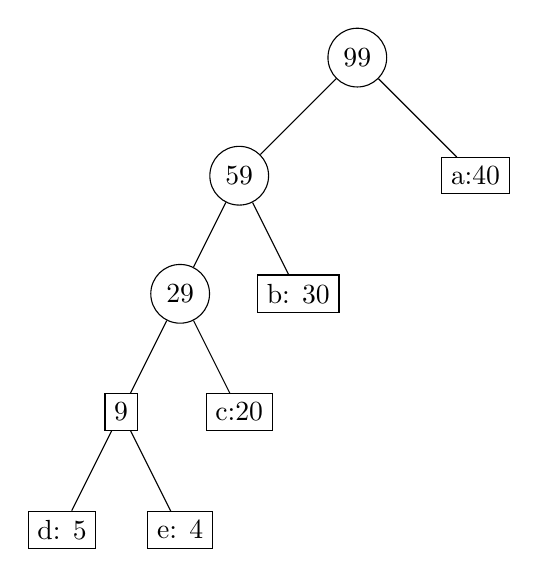
\begin{tikzpicture}[level distance=1.5cm,  level 1/.style={sibling distance=3cm},  level 2/.style={sibling distance=1.5cm}]
        \node [circle, draw] {99}
          child {node [circle, draw] {59}
            child {node [circle, draw] {29}
              child {node [rectangle, draw] {9}
                child {node [rectangle, draw] {d: 5}}
                child {node [rectangle, draw] {e: 4}}
              }
              child {node [rectangle, draw] {c:20}}
            }
            child {node [rectangle, draw] {b: 30}}
          }
          child {node [rectangle, draw] {a:40}
          };
      \end{tikzpicture}
\end{center}
}

\pageshift

\question{Matrix-chain multiplication}
The algorithm {\sc Matrix-Chain-Order}$(p,n)$ from CLRS 14.2 returns two arrays $m$ and $s$.
%Recall that the table $s$ indicates how to parenthesize a product of matrices $A_1A_2\cdots A_n$ so that it can be computed with the fewest multiplications.
%If $s[i,j]=k$, this means that the outermost parentheses in the product $A_i\cdots A_j$ should be placed as $(A_i\cdots A_k)(A_{k+1}\cdots A_j)$.
%
Below is an array $s[1:n-1, 2:n]$ returned by {\sc Matrix-Chain-Order}$(p,n)$ for a product of $n=6$ matrices $A_1\cdots A_6$ with dimensions given in $p$.
\medskip

\begin{tabular}{c|cccccc}
$i \backslash j$ & 2 & 3 & 4 & 5 & 6 \\
\hline
1 & 1 & 1 & 1 & 1 & 1 \\
2 & & 2 & 2 & 4 & 4 \\
3 &     & & 3 & 4 & 4 \\
4 &     &     & & 5 & 5 \\
5 &     &     &     & & 5 \\
\end{tabular}

\medskip\noindent
Give the parenthesization according to the table.
\oneanswer
%
\optionsstart
\answer $((A_1(A_2 A_3))((A_4 A_5)A_6))$

\answer $(A_1((A_2(A_3A_4))(A_5 A_6)))$ \correct

\answer $(((((A_1 A_2)A_3)A_4)A_5)A_6)$.

\answer $((((A_1 A_2)A_3)A_4)(A_5A_6))$.

\answer $((A_1(A_2 A_3))(A_4(A_5 A_6)))$
\optionsend
\explanation{Running the algorithm {\sc Print-Optimal-Parens}$(s,1,n)$ by hand gives the marked answer.}

\question{Paradigms}
Consider the following pseudocode, which takes an array $A$ and two indices $p$, $r$ as parameters.
\begin{codebox}
  \Procname{$\proc{MyRecursiveAlgorithm}(A, p, r)$}
  \li \If $p<r$ \Do
  \li $q = \lfloor (p+r)/2\rfloor$
  \li \If $A[p]>A[q]$ \Do
  \li \Return 0
  \li \Else
  \li $x = \proc{MyRecursiveAlgorithm}(A, p, q)$
  \li $y = \proc{MyRecursiveAlgorithm}(A, q+1, r)$
  \li \Return $\min(x,y)$ \End
  \li \Else
  \li \Return 1\End
\end{codebox}
Which of the paradigms below best describes $\proc{MyRecursiveAlgorithm}$?
\oneanswer
\optionsstart
\answer Divide and conquer \correct
\answer Dynamic programming
\answer Greedy algorithms
\optionsend
\explanation{The algorithm divides the problem into two smaller parts, solves them recursively and combines the results, which is characteristic of the divide-and-conquer paradigm.}

\question{Rotations in red-black search trees}
Consider this red-black search tree $T$, where the leaves are omitted:
\begin{center}
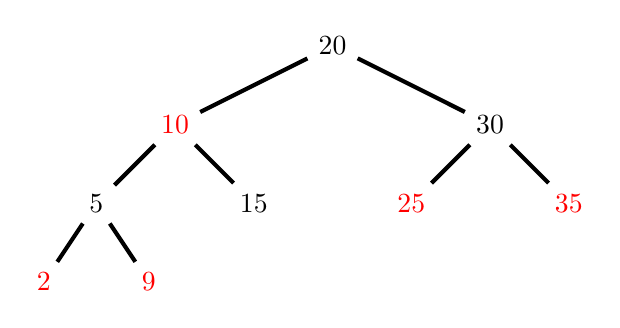
\begin{tikzpicture}[-,>=stealth,level/.style={sibling distance = 4cm/#1,
    level distance = 1cm}, line width=1.5pt]
  \node [black] {20}
      child{ node [red] {10}
              child{ node [black] {5}
                    child{ node [red] {2} }
                    child{ node [red] {9} }
              }
              child{ node [black] {15} }
      }
      child{ node [black] {30}
              child{ node [red] {25} }
              child{ node [red] {35} }
          }
  ;
  \end{tikzpicture}
\end{center}

\noindent
Suppose we run the algorithm {\sc Right-Rotate$(T,10)$} (cf.~CLRS Section 13.2) with the node $10$ as input. What happens to the tree $T$?
\multipleanswers
\optionsstart
\answer 9 becomes the left child of 10 \correct
\answer 10 becomes the right child of 5 \correct
\answer The height of the tree increases by 1
\answer The height of the tree remains unchanged \correct
\optionsend
\explanation{After a right rotation on the node $10$, the node $5$ moves up, and $10$ becomes its right child. The height of the tree remains the same, since 10's subtree is shorter than 5's subtrees.}

\question{Shortest paths}
In this problem we are interested in shortest paths in a graph with $n$ vertices, where each vertex has an edge to $d$ other vertices, where $2\leq d < n$.
Each edge has a nonnegative weight.
We want to use Dijkstra's algorithm to find shortest paths from a source vertex $s$ to all vertices in the graph.
Assume that the algorithm is implemented with a Fibonacci heap as the priority queue.
What can we say about the asymptotic running time as a function of $n$ and $d$?
\multipleanswers

\optionsstart
\answer The time is $O(nd + n \log d)$
\answer The time is $O(nd + n \log n)$ \correct
\answer The time is $O(nd + d \log d)$
\answer The time is $O(nd \log d)$
\answer The time is $O(n^2)$\correct
\answer The time is $O(n^2 \log d)$ \correct
\optionsend
\explanation{ The running time of Dijkstra's algorithm implemented with Fibonacci heaps is $O(n \log(n) + m)$, where $m$ is the number of edges.
In the situation described, $m=dn$, which means that the running time is $O(nd + n \log n)$.
Since $d < n$, this implies that the bound $O(n^2)$ is valid, and since $\log d \geq \log 2 > 0$, the bound $O(n^2 \log d)$ is also valid.
If $d=O(1)$, the three other bounds are $O(nd)$, linear in the number of edges, which is faster than Dijkstra's algorithm, which on worst-case graphs with $O(n)$ edges runs in time $\Theta(n \log n)$.
}

\pageshift

\question{Minimum spanning tree}
Consider the minimum spanning tree problem on the graph below:
\begin{center}
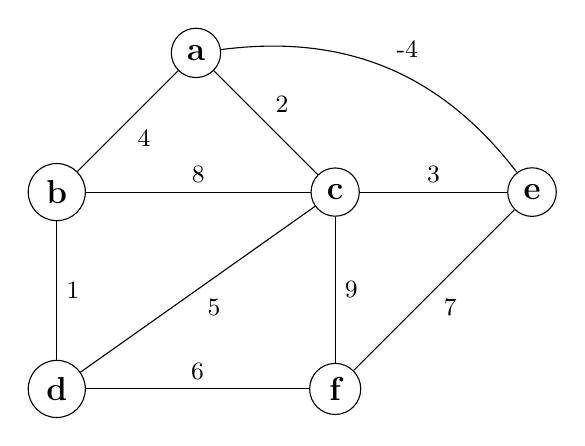
\begin{tikzpicture}[node distance=2.5cm, auto,>=stealth,
  main node/.style={circle,draw,font=\large\bfseries}]
  \node[main node] (a) {a};
  \node[main node] (b) [below left of=a] {b};
  \node[main node] (c) [below right of=a] {c};
  \node[main node] (d) [below of=b] {d};
  \node[main node] (e) [right of=c] {e};
  \node[main node] (f) [below of=c] {f};

  \path[every node/.style={font=\small}]
    (a) edge node {2} (c)
    (a) edge node {4} (b)
    (a) edge[bend left=30] node {-4} (e)
    (b) edge node {1} (d)
    (c) edge node {3} (e)
    (c) edge node {9} (f)
    (d) edge node {6} (f)
    (e) edge node {7} (f)
    (c) edge node {5} (d)
    (b) edge node {8} (c);
\end{tikzpicture}
\end{center}
Which edges are in the unique minimum spanning tree (MST)?
\multipleanswers
\optionsstart
\answer \{a,b\} \correct
\answer \{a,c\} \correct
\answer \{a,e\} \correct
\answer \{b,c\}
\answer \{b,d\} \correct
\answer \{c,d\}
\answer \{c,e\}
\answer \{c,f\}
\answer \{d,f\} \correct
\answer \{e,f\}
\optionsend
\explanation{Running Kruskal's algorithm, the edges are selected in increasing order: \(\{a,e\}\) (weight -4), \(\{b,d\}\) (weight 1), \(\{a,c\}\) (weight 2), \(\{a,b\}\) (weight 4 ) and \(\{d,f\}\) (weight 6). The other edges would create a cycle. Prim's algorithm gives the same answer, since the edge weights are distinct.}

\question{Graph algorithms}
Suppose you have an undirected, weighted graph with edge weights between $-100$ and $+100$.
The number of vertices is $n$ and the number of edges is $\binom{n}{2}$, i.e.,~every pair of vertices is connected by an edge with weight between $-100$ and $100$.
Which of the algorithms from CLRS below is the best choice for computing a minimum spanning tree (MST)?
\oneanswer
\optionsstart
\answer Breadth-first search
\answer The Bellman-Ford algorithm
\answer Dijkstra's algorithm
\answer Kruskal's algorithm \correct
\optionsend

\explanation{Among the algorithms listed, only one, namely Kruskal's algorithm, returns a minimum spanning tree. The others return \emph{shortest-paths trees} for various kinds of weighted, directed graphs. It does not matter that the weights can be negative or that the graph is complete.
%, but we note that Prim's algorithm with Fibonacci heaps is particularly efficient on graphs with many edges.
}

\question{Convex hulls}
Let $Q$ be a finite set of points in the plane.
Recall that $\text{CH}(Q)$ denotes the convex hull of $Q$.
Which statements are correct for \emph{every} such set $Q$?
\multipleanswers
\optionsstart
\answer $Q\subseteq\text{CH}(Q)$.\correct
\answer $\text{CH}(Q)$ is a triangle.
\answer Every vertex of $\text{CH}(Q)$ is a point in $Q$.\correct
\answer Every point in $Q$ is a vertex of $\text{CH}(Q)$.
\answer The point $(0,0)$ is in $\text{CH}(Q)$.
\answer The vertices of $\text{CH}(Q)$ can be computed in time $O(n/\log n)$, where $n$ is the number of points in $Q$.
\optionsend

\explanation{By definition, $Q\subseteq \text{CH}(Q)$. $\text{CH}(Q)$ can have many more vertices than a triangle.
$\text{CH}(Q)$ is a convex polygon with vertices in $Q$.
There are usually points in $Q$ that are not vertices of $\text{CH}(Q)$.
The point $(0,0)$ need not be in $\text{CH}(Q)$.
It is impossible to compute $\text{CH}(Q)$ in $O(\frac n{\log n})$ time, since such an algorithm does not even have time to read the coordinates of all the points, and so the algorithm cannot compute $\text{CH}(Q)$ correctly in all cases.}


\multiplechoiceend

\newpage

\section*{Written problems}\label{sec:written}

% Machine translated from the Danish original, ../danish/skriftlige.tex
{\bf Written problems:} \placeholder{How the answers are submitted, e.g.\ the file format and exam system, and whether drawings made on a tablet may be inserted.}
\begin{itemize}
    \item Use \emph{one page for each subquestion, in the same order as in the problem set.}
    \item The number/letter of the subquestion (e.g.\ 19 or 20.a) must be stated.
\end{itemize}


\section{Recursion and proofs by induction (10\%)}

Consider the following function, in the pseudocode notation of CLRS, where the input $A[1:n]$ is an array of \emph{distinct} integers and $x$ is an integer parameter.
We say that $A$ is \emph{bitonic} if there exists an index $m \in \{1,\dots,n\}$ such that $A[i] < A[i+1]$ for $1 \leq i < m$ and $A[i] > A[i+1]$ for $m\leq i < n$, i.e.,~if $A$ consists of an increasing sequence followed by a decreasing sequence.
In this problem the following recursive function is to be analyzed:

\begin{codebox}
\Procname{$\proc{BTS}(A, p, q, x)$}
\li \If $p > q$ \Return \textbf{false}
\li $mid \gets \lfloor (p+q)/2 \rfloor$
\li \If $A[mid] == x$ \Return \textbf{true}
\li \ElseIf $p==q$ \Return \textbf{false}
\li \If $(A[mid] > A[mid+1]) \textbf{ or } (x < A[mid])$
\li \Then $L \gets \proc{BTS}(A, p, mid-1, x)$
\li \Else $L \gets$ \textbf{false}\End
\li \If $(A[mid] < A[mid+1]) \textbf{ or } (x < A[mid])$
\li \Then $R \gets \proc{BTS}(A, mid+1, q, x)$
\li \Else $R \gets$ \textbf{false} \End
\li \Return $L$ \textbf{ or } $R$
\end{codebox}

\noindent
{\bf Example:} If $n=8$ and $A = \langle 2, 3, 5, 7, 11, 8, 4, 1\rangle$, then $\proc{BTS}(A, 1, n, 5)$ returns the value {\bf true}, while $\proc{BTS}(A, 1, n, 6)$ returns the value {\bf false}.
\medskip

\subquestion{a)}{ Explain in words what $\proc{BTS}(A, 1, n, x)$ returns if $A[1:n]$ is bitonic, without repeated elements, and $x$ is an arbitrary integer. You do not need to justify your answer in this subquestion. }

\explanation{ $\proc{BTS}(A, 1, n, x)$ returns {\bf true} if the element $x$ is in $A$, and {\bf false} otherwise. (This is because the algorithm exploits the bitonic property to select which subarrays cannot contain $x$.) }

\subquestion{b)}{ Give an example of an input $A$ and $x$, where $A$ contains $n$ distinct integers in arbitrary order, for which $\proc{BTS}(A, 1, n, x)$ does not return the same as it would if the elements of $A$ had been in a bitonic order, e.g., sorted.}

\explanation{ If $A = \langle 2, 1, 3\rangle$ (not bitonic) and $x=2$, {\bf false} is returned, but for $A = \langle 1, 2, 3\rangle$ (bitonic) and $x=2$, {\bf true} is returned.}

\subquestion{c)}{ Give a proof by induction of the claim in a). }

\explanation{ We want to show that $\proc{BTS}(A, p, q, x)$ returns {\bf true} if and only if $x$ is in $A[p:q]$. Setting $p=1$ and $q=n$ gives the claim in a).
The proof is by induction on the length of the subarray, $n = q - p + 1$. The case $n=0$ is covered by line~1 (the subarray is empty), and the case $n=1$ is covered by line~3 (the subarray has length~1).
Assume that the claim is true for subarrays of length $n' < n$ (induction hypothesis), and consider a subarray of length $n$.
If $A[mid]=x$, line~3 gives the desired result if $x$ is at index $mid$.
Otherwise, we note that the result of comparing $A[mid]$ and $A[mid+1]$ tells us whether $mid$ and $mid+1$ lie in the increasing or the decreasing part of $A$.
This means that a recursive call is made on $A[p:mid-1]$ if it is possible that $x$ is there (lines 5--6), and on $A[mid+1:q]$ if it is possible that $x$ is there (lines 8--9).
By the induction hypothesis, $L$ is therefore set to {\bf true} exactly if $x$ is in the left part, and $R$ is set to {\bf true} exactly if $x$ is in the right part.
Finally, the logical {\bf or} of the two values is returned. This completes the inductive step.}


\section{Room allocation (9\%)}

A university is trying to hold exams in as many courses as possible on the afternoon of 31~March 2025.
There are $n$ courses whose sizes, measured in number of students, are represented as an array $S[1:n]$.
There are $m$ exam rooms available, whose capacities are represented as an array $K[1:m]$.
Course $i$ can be held in room $j$ if and only if $S[i]\leq K[j]$.
Each room can hold the exam of at most one course, and each course has its exam in at most one room.
We assume that both $S$ and $K$ are sorted in nondecreasing order.

\medskip

\textbf{Example:}
Let $S=\langle 25, 150, 300\rangle$ be the numbers of students in the courses CG, Inter and AD, respectively.
Let $K=\langle 50, 500\rangle$ be the capacities of the two available rooms.
We can then hold the CG exam in room $1$ and the AD exam in room $2$, and the Inter exam has to be held at another time.

\subquestion{a)}{Let $S=\langle 18,45,153,354,503\rangle$ and $K=\langle20,20,50,75,200,400,400\rangle$.
Give an allocation of courses to rooms such that we hold as many exams as possible.}

\explanation{We can hold exams in four of the courses, e.g., course $1$ in room $1$, course $2$ in room $3$, course $3$ in room $5$ and course $4$ in room $6$.
Course $5$ cannot be held, since it is too large for all rooms.}

\subquestion{b)}{Prove or disprove the following statement: Let $t$ be the maximum number of courses for which we can hold an exam.
There exists an allocation of rooms in which we hold exams in courses $1,\ldots,t$, that is, the $t$ smallest courses, and these have been allocated rooms in sorted order, i.e.,~if courses $i$ and $i+1$ have been allocated rooms $j_1$ and $j_2$, then $j_1<j_2$.}

\explanation{The statement is true.
If we have not allocated rooms to the $t$ smallest courses, we can replace the largest allocated course by the smallest unallocated course, and we can keep doing this until we have allocated the $t$ smallest.
Furthermore, if courses $i$ and $i+1$ have been allocated rooms $j_1$ and $j_2$ with $j_1>j_2$, we can swap the rooms of courses $i$ and $i+1$, so that the small course gets the small room and the large course gets the large room.}

\subquestion{c)}{Describe an algorithm for finding the maximum number of courses for which we can hold an exam.
You may write pseudocode, but a clear and precise description in text is also sufficient.
To get full points, you must account for correctness and for the running time being linear.}

\explanation{The problem can be solved with a greedy algorithm:

\begin{codebox}
\Procname{$\proc{ExamAllocation}(K, S)$}
\li $i \gets 1$
\li $j \gets 1$
\li $a \gets 0$
\li \While $i \leq n$ \textbf{ and } $j \leq m$ \Do
\li \quad \While $j \leq m$ \textbf{ and } $S[i] > K[j]$ \Do
\li \quad\quad $j \gets j + 1$ \End
\li \quad \If $j \leq m$ \Then
\li \quad\quad $a \gets a + 1$
\li \quad\quad $i \gets i + 1$
\li \quad\quad $j \gets j + 1$ \End \End
\li \Return $a$
\end{codebox}

Explanation in text: We consider the courses in sorted order and, for each course, greedily choose the smallest room that is large enough and has not already been used.
This can be implemented with indices $i$ and $j$ into the courses and the rooms, respectively.
At the beginning of each iteration, course $i$ is the smallest course that has not been given a room, and room $j$ is the smallest room that has not been used yet and that is large enough for the preceding course $i-1$.
As long as $S[i]> K[j]$ and $j\leq m$, we increment $j$.
The case $j==m+1$ corresponds to having no rooms left that are large enough for course $i$, so we stop.
If, on the other hand, $S[i]\leq K[j]$, we allocate course $i$ to room $j$ and increment a variable $a$, which counts how many courses we have allocated rooms to.
We also increment both $i$ and $j$ and are ready for the next iteration.
We stop if $i==n+1$, which corresponds to having allocated rooms to all courses.
Finally, we return the value $a$.

In total we go through $K$ and $S$ at most once each, so the running time is $O(n+m)$.
}



\section{Cake optimization (9\%)}\label{sec:last}

Professor Sweettooth is both genial and very sociable, and is therefore invited to a birthday party every single day, $n$ days in a row, at different friends' homes.
The professor's doctor has strongly advised against going to birthday parties two days in a row, since one ends up overeating on cake.
Professor Sweettooth knows his friends well, and therefore knows exactly how good the cakes they bake are.
The professor defines an array $K[1:n]$ such that $K[i]$ is a positive integer indicating how good the cakes one can expect to be served at the birthday party on day $i$ are.
The professor now wants to select a set $I\subset\{1,2,\ldots,n\}$ that complies with the doctor's advice, i.e.,~if $i\in I$ then $i+1\notin I$, and such that the total quality of the cakes, $\sum_{i\in I} K[i]$, is maximized.

\subquestion{a)}{Professor Sweettooth makes the following hypothesis:
If, in an optimal solution, one attends the birthday party on day $i\leq n-3$, then one must also go on day $i+2$ or $i+3$.
Is the hypothesis correct?
Give a proof or a counterexample.}

\explanation{Suppose that one takes a break of three days or more after day $i$.
Then one can also go on day $i+2$ without violating the doctor's advice, and thereby get more cake.
Since all cakes have positive value, this is a contradiction, and therefore the statement holds.}

\subquestion{b)}{Professor Sweettooth now considers an alternative hypothesis:
Regardless of the values in $K$, there is an optimal solution in which one goes to a birthday party every other day, i.e., either on days $1,3,5,\ldots$ or on days $2,4,6,\ldots$.
Is the hypothesis correct?
Give a proof or a counterexample.}

\explanation{If $K=\langle 10,1,1,10\rangle$, it is best to go to the birthday parties on days $1$ and $4$, so the hypothesis is false.}

\subquestion{c)}{Describe an algorithm that can compute the maximum sum $\sum_{i\in I} K[i]$.
You may write pseudocode, but a clear and precise description in text is also sufficient.
To get full points, you must account for correctness and for the running time being $O(n)$.}

\explanation{For $i\geq 0$ we let $S_i$ be the maximum sum over the days $1,2,\ldots,i$, where we define $S_0=0$.
We explain how we can find all the values $S_0,S_1,\ldots,S_n$ in $O(n)$ time using dynamic programming.
Note that $S_n$ is the maximum sum asked for in the problem.

The base cases are $S_0=0$ and $S_1=K[1]$.
If one goes to the birthday party on day $i\geq 2$, then day $i-1$ is a rest day, and therefore we have $S_i=S_{i-2}+K[i]$.
If one stays at home on day $i$, then we have $S_i=S_{i-1}$.
Therefore $S_i=\max\{S_{i-2}+K[i],S_{i-1}\}$.
With this formula we can find $S_2,\ldots,S_n$ in $O(n)$ time by iterating through the values $i=2,\ldots,n$.

\begin{codebox}
\Procname{$\proc{CakeOptimization}(K, n)$}
\li let $S[0:n]$ be a new array
\li $S[0] \gets 0$
\li $S[1] \gets K[1]$
\li \For $i \gets 2$ \To $n$ \Do
\li \quad $S[i] \gets \max(S[i-2] + K[i], S[i-1])$ \End
\li \Return $S[n]$
\end{codebox}
}

\label{page:last}
